\documentclass[11pt]{article}
\usepackage{geometry,marginnote} % Pour passer au format A4
\geometry{hmargin=1cm, vmargin=1.5cm} % 

% Page et encodage
\usepackage[T1]{fontenc} % Use 8-bit encoding that has 256 glyphs
\usepackage[english,french]{babel} % Français et anglais
\usepackage[utf8]{inputenc} 

\usepackage{lmodern}
\usepackage[np]{numprint}
\setlength\parindent{0pt}

% Graphiques
\usepackage{graphicx,float,grffile}
\usepackage{tikz,pst-eucl,pst-plot,pstricks,pst-node,pstricks-add,pst-fun,pgfplots} 

% Maths et divers
\usepackage{amsmath,amsfonts,amssymb,amsthm,verbatim,scratch3}
\usepackage{multicol,enumitem,url,eurosym,gensymb,tabularx}

\DeclareUnicodeCharacter{20AC}{\euro}



% Sections
\usepackage{sectsty} % Allows customizing section commands
\allsectionsfont{\centering \normalfont\scshape}

% Tête et pied de page
\usepackage{fancyhdr} \pagestyle{fancy} \fancyhead{} \fancyfoot{}

%\fancyfoot[L]{Collège Faubert}
%\fancyfoot[C]{\thepage / 6}
%\fancyfoot[R]{Série Générale}

\renewcommand{\headrulewidth}{0pt} % Remove header underlines
%\renewcommand{\footrulewidth}{0pt} % Remove footer underlines

\newcommand{\horrule}[1]{\rule{\linewidth}{#1}} % Create horizontal rule command with 1 argument of height

\newcommand{\Pointilles}[1][3]{%
  \multido{}{#1}{\makebox[\linewidth]{\dotfill}\\[\parskip]
}}

\newtheorem{Definition}{Définition}

\usepackage{siunitx}
\sisetup{
    detect-all,
    output-decimal-marker={,},
    group-minimum-digits = 3,
    group-separator={~},
    number-unit-separator={~},
    inter-unit-product={~}
}

\setlength{\columnseprule}{1pt}


\begin{document}

\textbf{Nom, Prénom :} \hspace{8cm} \textbf{Classe :} \hspace{3cm} \textbf{Date :}\\

\begin{center}
  \textit{Le plus grand ennemi de la connaissance n'est pas l'ignorance. C'est l'illusion de la connaissance.} 
  
  \textbf{Stephen Hawking}
\end{center}


\subsection*{Définitions}
  \begin{enumerate}
    \item[1.] Nombre négatif : \dotfill \\
    \Pointilles[1]
    \item[2.] Pourquoi doit-on écrire la phrase réponse après les calculs ?  \dotfill \\
    \Pointilles[2]
  \end{enumerate}

\subsection*{Exercice 1 - Calculer}

\begin{multicols}{3}\noindent
  \begin{itemize}[label={$\bullet$}]
        \item $-40 \div \ldots\ldots = -10$
        \item $\ldots\ldots \div \left( -6\right) = -1$
        \item $\ldots\ldots + 9 = -5$
        \item $\ldots\ldots + \left( - 12\right) = -2$
        \item $-44 \div 11 = \ldots\ldots$
        \item $-60 \div \ldots\ldots = 10$
        \item $-7 - 7 = \ldots\ldots$
        \item $\ldots\ldots \times 10 = -50$
        \item $-10 - 1 = \ldots\ldots$
        \item $-4 \times 8 = \ldots\ldots$
        \item $\ldots\ldots - \left( -4\right) = -8$
        \item $-1 \div -1 = \ldots\ldots$
    \end{itemize}
  \end{multicols}

\subsection*{Exercice 2 - Calculer}

\begin{itemize}[label={$\bullet$}]
        \item $-70 \times \dfrac{-15 - 145}{25 - 3 \times 32} + -4300 - \dfrac{3500}{-27} \simeq $ \dotfill
\end{itemize}


\subsection*{Problèmes}

\begin{minipage}[t]{0.25\textwidth}
  \begin{figure}[H]
    \centering
    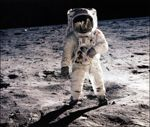
\includegraphics[width=100px]{4x2-nombres-relatifs/ex1.jpg}
  \end{figure}
\end{minipage}
\begin{minipage}[t]{0.75\textwidth}
\textbf{1.} Neil Armstrong de l'équipage d'Appolo 11 est sorti du module lunaire le 20 juillet 1969 pour faire le premier pas de l'Homme sur la Lune. La température sur la lune était de $-21 \degree C$. Sa combinaison était chauffée à une température de $32 \degree C$. 

Quelle était la différence de température entre l'intérieur et l'extérieur de sa combinaison ? \\
\Pointilles[6]
\end{minipage}

\begin{minipage}[t]{0.25\textwidth}
  \begin{figure}[H]
    \centering
    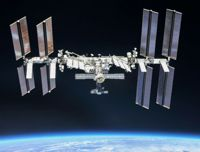
\includegraphics[width=100px]{4x2-nombres-relatifs/ex4.jpg}
  \end{figure}
\end{minipage}
\begin{minipage}[t]{0.75\textwidth}
  \textbf{2.} Sur Mars, la température le jour est de $27\degree C$ et la nuit de $-84\degree C$. Quelle est la différence de température entre le jour et la nuit ?\\
  \Pointilles[6]
\end{minipage}

\newpage

\begin{minipage}[t]{0.25\textwidth}
  \begin{figure}[H]
    \centering
    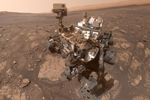
\includegraphics[width=100px]{4x2-nombres-relatifs/ex5.jpg}
  \end{figure}
\end{minipage}
\begin{minipage}[t]{0.75\textwidth}
  \textbf{3.} Le robot Curiosity relève les températures tous les jours. Aujourd'hui Il note un minimum a $-56 \degree C$. Il note un écart de température de $ 109\degree C$. Mais la température maximum ne s'est pas enregistrée car il y avait une tempête de sable au moment de la transmission. Peut-on quand même connaître cette température maximale ?\\
  \Pointilles[3]
\end{minipage}

\Pointilles[2]

\begin{minipage}[t]{0.25\textwidth}
  \begin{figure}[H]
    \centering
    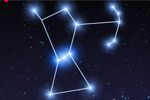
\includegraphics[width=100px]{4x2-nombres-relatifs/ex7.jpg}
  \end{figure}
\end{minipage}
  \begin{minipage}[t]{0.75\textwidth}
    \textbf{4.} Des scientifiques utilisent le télescope James Web (JWST) pour étudier la constellation d'Orion.
  \begin{itemize}
    \item La température de Rigel est de 21 900K.
    \item La température de notre Soleil est de 6600K.
    \item La température de Betelgeuse est trois fois plus chaude que notre Soleil.
  \end{itemize}
  L'astronome Didier Queloz pense que Betelgeuse est plus froide que Rigel. A-t-il raison ? \\
\end{minipage}

\Pointilles[7]

\begin{minipage}[t]{0.25\textwidth}
  \begin{figure}[H]
    \centering
    
\includegraphics[width=100px]{4x2-nombres-relatifs/ex2.jpg}
  \end{figure}
\end{minipage}
\begin{minipage}[t]{0.75\textwidth}
  \textbf{5.} Dans FF7, votre personnage Cloud vient de subir une magie poison. Il s'affiche à l'écran -17HP toutes les 7 secondes. Sachant qu'il est au niveau 7 et possède 2402HP, combien de temps peut-il survivre ?\\
  \Pointilles[6]
\end{minipage}

\Pointilles[3]

\begin{minipage}[t]{0.25\textwidth}
  \begin{figure}[H]
    \centering
    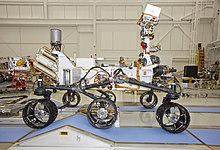
\includegraphics[width=100px]{4x2-nombres-relatifs/ex3.jpg}
  \end{figure}
\end{minipage}
\begin{minipage}[t]{0.75\textwidth}
  \textbf{6.} Dans Zelda, Link a le choix entre trois armes : 
  \begin{itemize}
    \item l'épée inflige 126 dégâts toutes les 6 secondes.
    \item La hache inflige 190 dégâts toutes les 10 secondes.
    \item La dague inflige 20 dégâts toutes les secondes.
  \end{itemize}
  Quelle arme est la plus efficace sur un temps de 1min ?\\
  \Pointilles[5]
\end{minipage}

\Pointilles[3]

\newpage

\textbf{Nom, Prénom :} \hspace{8cm} \textbf{Classe :} \hspace{3cm} \textbf{Date :}\\

\begin{center}
  \textit{Le plus grand ennemi de la connaissance n'est pas l'ignorance. C'est l'illusion de la connaissance.} 
  
  \textbf{Stephen Hawking}
\end{center}


\subsection*{Définitions}
  \begin{enumerate}
    \item[1.] Nombre négatif : \dotfill \\
    \Pointilles[1]
    \item[2.] Pourquoi doit-on écrire la phrase réponse après les calculs ?  \dotfill \\
    \Pointilles[2]
  \end{enumerate}

\subsection*{Exercice 1 - Calculer}

\begin{multicols}{3}\noindent
  \begin{itemize}[label={$\bullet$}]
        \item $-30 \div \ldots\ldots = 10$
        \item $\ldots\ldots \div \left( -6\right) = -1$
        \item $\ldots\ldots + 8 = -10$
        \item $\ldots\ldots + \left( -16\right) = -1$
        \item $-30 \div -3 = \ldots\ldots$
        \item $-120 \div \ldots\ldots = 10$
        \item $-8 - 8 = \ldots\ldots$
        \item $\ldots\ldots \times 10 = -40$
        \item $-15 - 5 = \ldots\ldots$
        \item $-5 \times 7 = \ldots\ldots$
        \item $\ldots\ldots - \left( -1\right) = -4$
        \item $-1 \div -1 = \ldots\ldots$
    \end{itemize}
  \end{multicols}

\subsection*{Exercice 2 - Calculer}

\begin{itemize}[label={$\bullet$}]
        \item $-35 \times \dfrac{-50 - 45}{252 - 4 \times 52} + -3500 - \dfrac{6200}{-97} \simeq $ \dotfill
\end{itemize}


\subsection*{Problèmes}

\begin{minipage}[t]{0.25\textwidth}
  \begin{figure}[H]
    \centering
    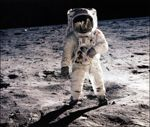
\includegraphics[width=100px]{4x2-nombres-relatifs/ex1.jpg}
  \end{figure}
\end{minipage}
\begin{minipage}[t]{0.75\textwidth}
\textbf{1.} Neil Armstrong de l'équipage d'Appolo 11 est sorti du module lunaire le 20 juillet 1969 pour faire le premier pas de l'Homme sur la Lune. La température sur la lune était de $-175 \degree C$. Sa combinaison était chauffée à une température de $28 \degree C$. 

Quelle était la différence de température entre l'intérieur et l'extérieur de sa combinaison ? \\
\Pointilles[6]
\end{minipage}

\begin{minipage}[t]{0.25\textwidth}
  \begin{figure}[H]
    \centering
    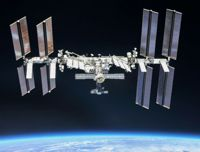
\includegraphics[width=100px]{4x2-nombres-relatifs/ex4.jpg}
  \end{figure}
\end{minipage}
\begin{minipage}[t]{0.75\textwidth}
  \textbf{2.} Sur Mars, la température le jour est de $17\degree C$ et la nuit de $-152\degree C$. Quelle est la différence de température entre le jour et la nuit ?\\
  \Pointilles[6]
\end{minipage}

\newpage

\begin{minipage}[t]{0.25\textwidth}
  \begin{figure}[H]
    \centering
    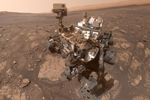
\includegraphics[width=100px]{4x2-nombres-relatifs/ex5.jpg}
  \end{figure}
\end{minipage}
\begin{minipage}[t]{0.75\textwidth}
  \textbf{3.} Le robot Curiosity relève les températures tous les jours. Aujourd'hui Il note un minimum a $-86 \degree C$. Il note un écart de température de $ 152\degree C$. Mais la température maximum ne s'est pas enregistrée car il y avait une tempête de sable au moment de la transmission. Peut-on quand même connaître cette température maximale ?\\
  \Pointilles[3]
\end{minipage}

\Pointilles[2]

\begin{minipage}[t]{0.25\textwidth}
  \begin{figure}[H]
    \centering
    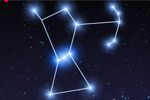
\includegraphics[width=100px]{4x2-nombres-relatifs/ex7.jpg}
  \end{figure}
\end{minipage}
  \begin{minipage}[t]{0.75\textwidth}
    \textbf{4.} Des scientifiques utilisent le télescope James Web (JWST) pour étudier la constellation d'Orion.
  \begin{itemize}
    \item La température de Rigel est de 21 300K.
    \item La température de notre Soleil est de 5400K.
    \item La température de Betelgeuse est quatre fois plus chaude que notre Soleil.
  \end{itemize}
  L'astronome Didier Queloz pense que Betelgeuse est plus froide que Rigel. A-t-il raison ? \\
\end{minipage}

\Pointilles[7]

\begin{minipage}[t]{0.25\textwidth}
  \begin{figure}[H]
    \centering
    
\includegraphics[width=100px]{4x2-nombres-relatifs/ex2.jpg}
  \end{figure}
\end{minipage}
\begin{minipage}[t]{0.75\textwidth}
  \textbf{5.} Dans FF7, votre personnage Cloud vient de subir une magie poison. Il s'affiche à l'écran -18HP toutes les 11 secondes. Sachant qu'il est au niveau 7 et possède 2536HP, combien de temps peut-il survivre ?\\
  \Pointilles[6]
\end{minipage}

\Pointilles[3]

\begin{minipage}[t]{0.25\textwidth}
  \begin{figure}[H]
    \centering
    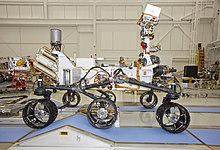
\includegraphics[width=100px]{4x2-nombres-relatifs/ex3.jpg}
  \end{figure}
\end{minipage}
\begin{minipage}[t]{0.75\textwidth}
  \textbf{6.} Dans Zelda, Link a le choix entre trois armes : 
  \begin{itemize}
    \item l'épée inflige 126 dégâts toutes les 6 secondes.
    \item La hache inflige 218 dégâts toutes les 10 secondes.
    \item La dague inflige 21 dégâts toutes les secondes.
  \end{itemize}
  Quelle arme est la plus efficace sur un temps de 1min ?\\
  \Pointilles[5]
\end{minipage}

\Pointilles[3]

\end{document}